\chapter{Seuil de rentablité}

Ce chapitre sera consacré à l'étude de problèmes financiers.

\section{Recherche de seuil}

Nous nous intéresserons ici aux entreprises qui produisent un seul article. Pour pouvoir en fabriquer en quantité, elles ont un certain nombre de frais.

Des frais sont liés à l'existence de l'entreprise (local à louer, machines à acheter, etc.) et d'autres à la production (matière première, etc). On appelle les premiers les \emph{frais fixes}\index{seuil de rentabilité!frais fixes}, notés $f_f$ et les second les \emph{frais variables}\index{seuil de rentabilité!frais variables}, notés $f_v$. Bien entendu, les frais fixes ne dépendent pas du nombre d'objets produits, alors que les second oui.

Secondement, l'entreprise vend ses produits, ce qui génère un \emph{gain}\index{seuil de rentabilité!gain}, noté $g$. L'ensemble des gains pour la vente de toute la production est ce qu'on appelle en économie le chiffre d'affaire. Dans tout ce chapitre, nous considérerons que l'ensemble de la production est systématiquement vendue.

Le \emph{seuil de rentabilité}\index{seuil de rentabilité} est le nombre d'objet qu'il faut produire afin d'équilibrer les gains et les frais. Il se trouve en résolvant l'équation

$$
f_v \cdot x + f_f = g\cdot x
$$
où $x$ est le nombre de marchandise produite. La fonction $f_v + f_f \cdot x$ représente l'ensemble des frais de l'entreprise pour produire $x$ marchandise, alors que la fonction $g\cdot x$ l'ensemble des gains liés à la vente de $x$ marchandises.

\begin{exemple}\label{ex_seuil}
Mon amie décide de se lancer dans la production de scoubidous. Pour cela, elle doit acheter une tresseuse de scoubidous à $100$ Frs. Elle a calculé que chaque scoubidou lui coûte $0.50$ Frs de fil. Enfin, elle décide de les vendre $3$ Frs pièce. Quel est sont seuil de rentabilité ?

En analysant le problème, on trouve :
$$
\left\{
\begin{array}{l}
f_f = 100\\
f_v = 0.5
g = 3
\end{array}
\right.
\Rightarrow
\left\{
\begin{array}{l}
f(x) = 0.5 x + 100\\
g(x) = 3x
\end{array}
\right.
$$
On doit donc résoudre l'équation
$$
\begin{array}{lcl}
0.5 x + 100 &=& 3x \ssi \\
100 &=& 2.5 x \ssi \\
40 &=& x
\end{array}
$$
Son seuil de rentabilité est donc de $40$ pièces, c'est-à-dire que si elle en produit moins elle perd de l'argent, et elle commence à en gagner à $41$ pièces.
\end{exemple}

\subsection{Représentation}

On vient de le voir, la situation peut être explicitée sous la forme de deux fonctions :
$$
\begin{array}{l}
f(x) = f_v \cdot c + f_f \mbox{ (les frais)}\\
g(x) = g\cdot x \mbox{ (les gains)}
\end{array}
$$

Or il s'agit de deux fonctions affines dont nous avons parlé à la section~\ref{fct_affine}. Puisque $x$ ne peut être que positif (il est peu probable de produite un nombre négatif de marchandise) et que les images des nombres positifs par $f$ et $g$ sont aussi positives, nous nous contenterons de représenter la situation dans le premier cadran, c'est-à-dire le quart supérieur droite.

Le seuil de rentabilité est le moment où $f(x) = g(x)$, et donc les deux graphes passent par le point $\left(x;f(x)\right) = \left(x;g(x)\right)$. Ainsi, puisque les deux droites passent par ce point, elle se coupent au seuil de rentabilité.

Pour une représentation un peu précise, il convient de représenter chaque droite en utilisant l'image de $0$ (l'ordonnée à l'origine) et l'image d'un nombre suffisamment grand (en général, deux fois le seuil de rentabilité).

\begin{exemple}
Reprenons l'exemple~\ref{ex_seuil} : nous avons les deux fonction suivantes :
$$
\left\{
\begin{array}{l}
f(x) = 0.5 x + 100\\
g(x) = 3x
\end{array}
\right.
$$
On sait déjà que le seuil est à $40$ pièces, nous allons donc calculer les images de $0$ et de $80$ :
$$
\left\{
\begin{array}{l}
f(0) = 0.5 \cdot 0 + 100 = 100 \Rightarrow (0;100)\\
g(0) = 3\cdot 0 = 0 \Rightarrow (0;0)
\end{array}
\right.
\mbox{ et }
\left\{
\begin{array}{l}
f(80) = 0.5 \cdot 80 + 100 = 140 \Rightarrow (0;140)\\
g(80) = 3\cdot 80 =240 \Rightarrow (0;240)
\end{array}
\right.
$$
On représente donc la situation ainsi :
\begin{center}
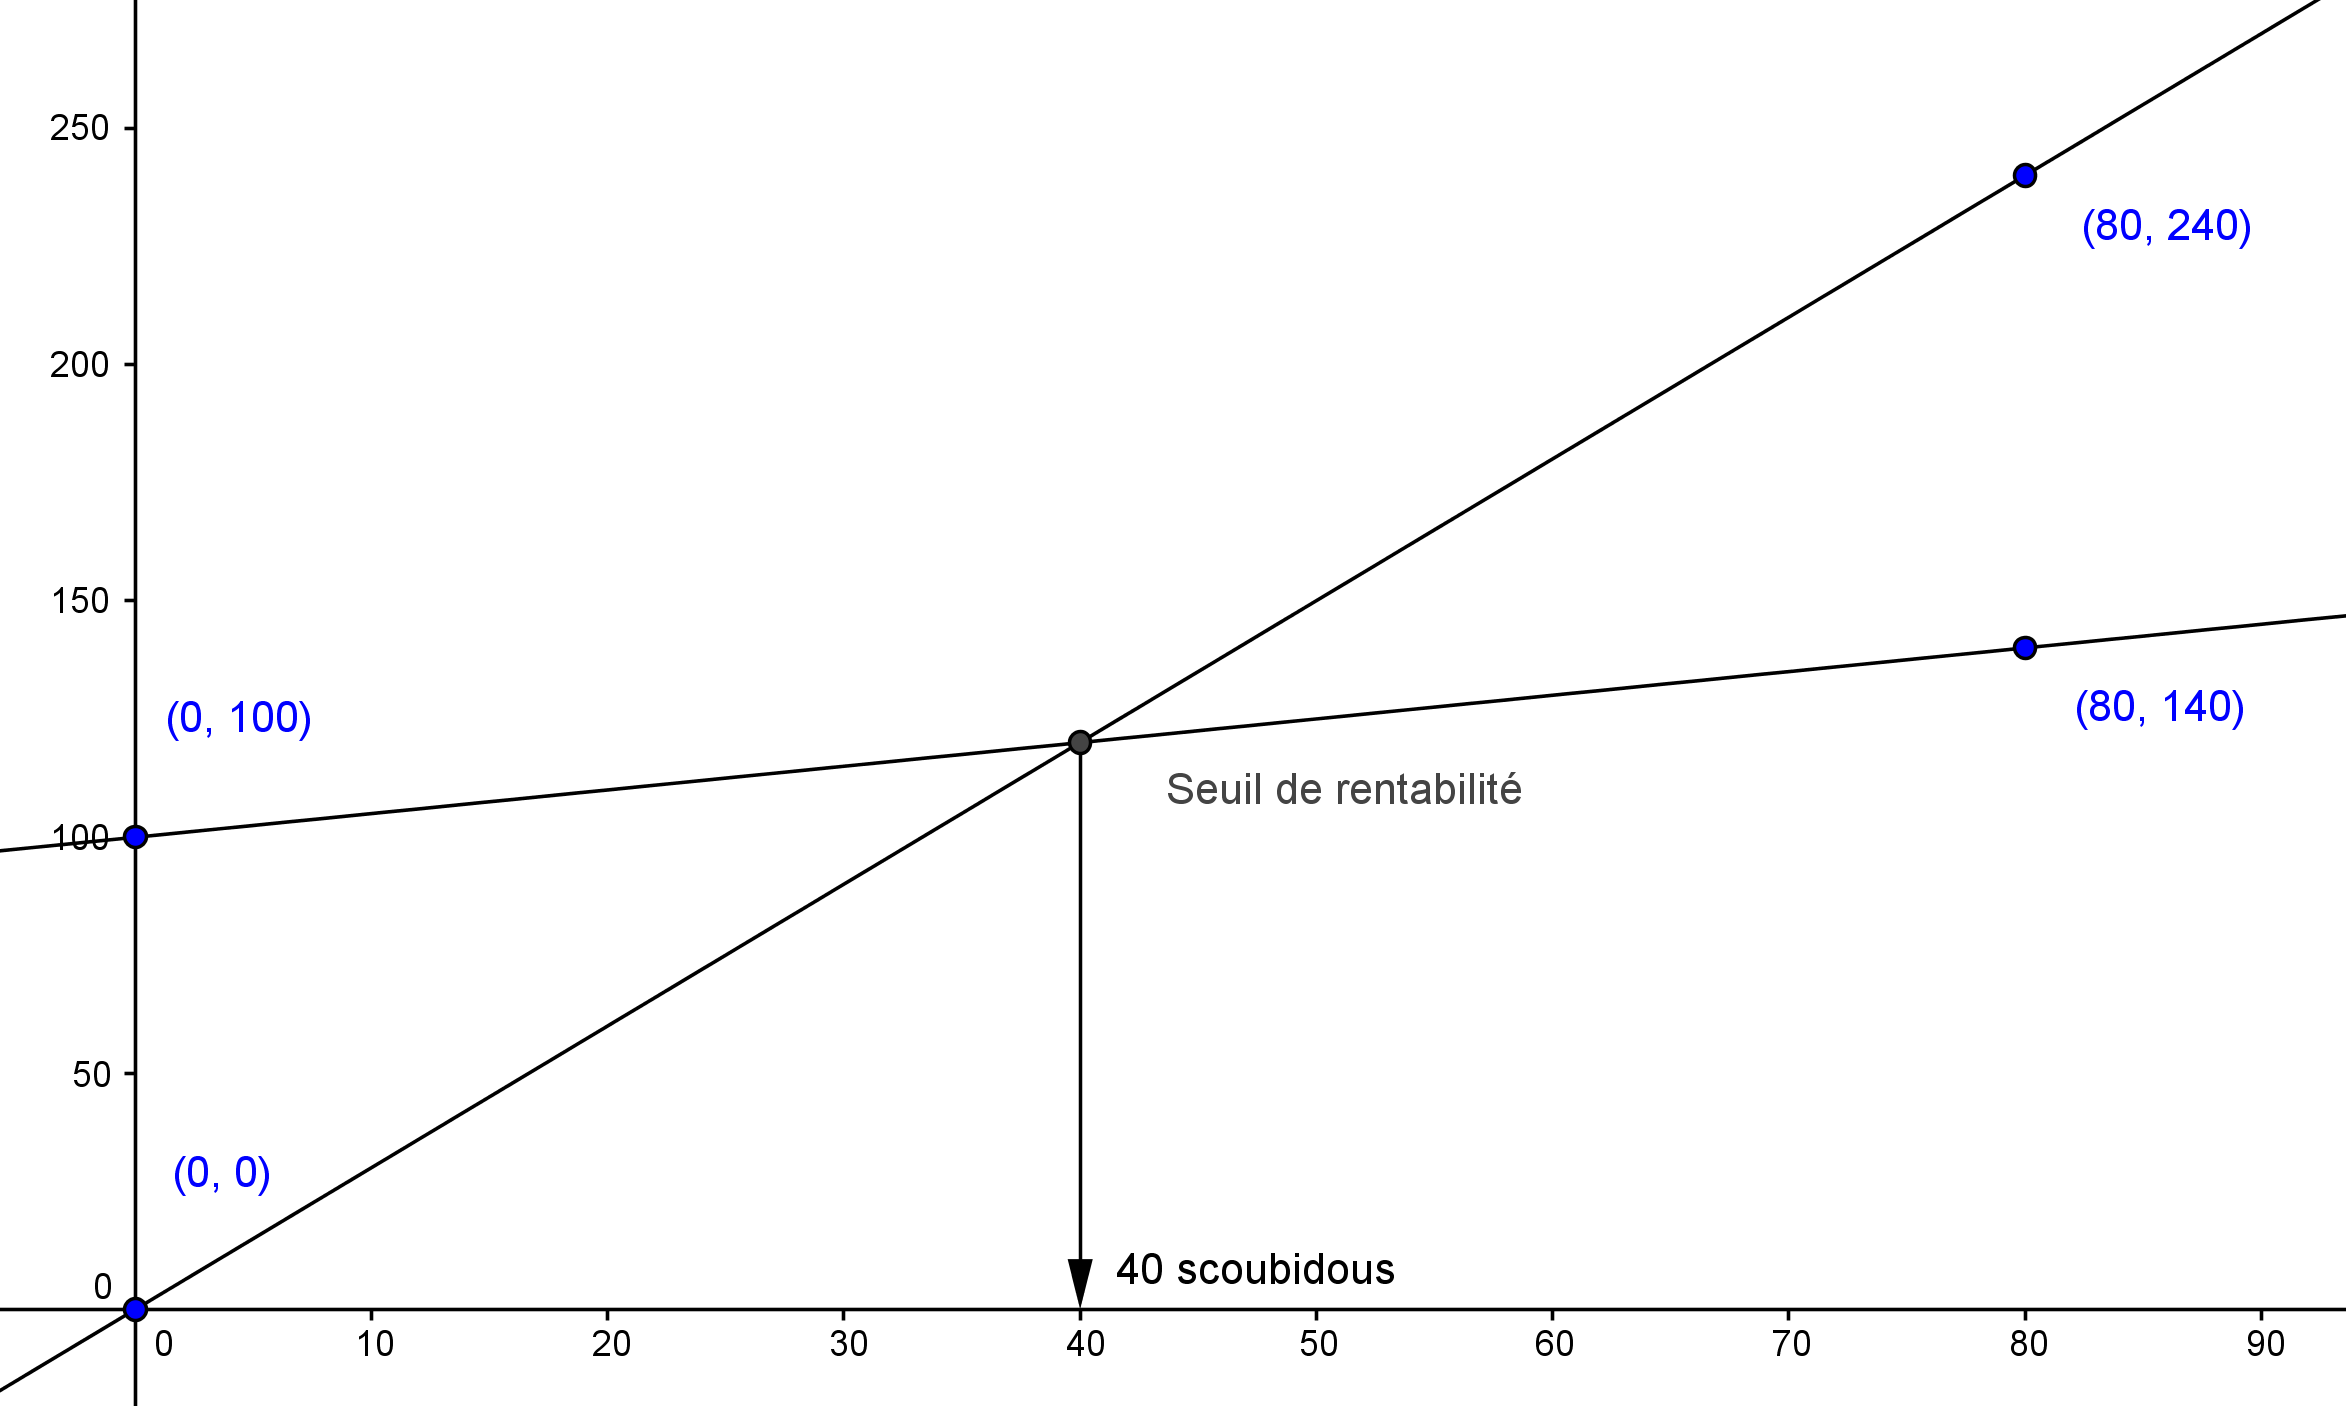
\includegraphics[width=0.7\textwidth]{rentabilite/seuil_ex.png}
\end{center}
Pour faciliter la représentation, il est souvent nécessaire de ne pas utiliser la même graduation pour les deux axes !
\end{exemple}

\section{Comparatif d'offres}

Cette section peut paraître n'avoir aucun lien avec le chapitre, mais le raisonnement est le même que pour les seuil de rentabilités.

On s'intéresse ici à plusieurs offres portant sur la même matière (par exemple : payer tous ses  trajets, prendre un demi-tarif ou un abonnement général) et on cherche à analyser l'offre. Par exemple, à partir de combien de trajet prendre un demi tarif est-il plus avantageux que de payer en plein chaque déplacement ?

Pour cela, nous allons commencer par décrire la fonction liée à chaque offre, représenter son graphe et nous intéresser aux points d'intersection (on commence à voir le rapport avec le seuil de rentabilité).

\begin{exemple}
Jean-Paul fait régulièrement le trajet Martigny-Genève. Il paye son billet $41$ Frs. Le demi-tarif est à $185$ Frs par année et l'abonnement général à $3655$ Frs par année. Que conseiller à Jean-Paul ?

Soit $x$ le nombre de trajets que Jean-Paul effectue par année, $h(x)$ ce qu'il paye avec des billets normaux, $i(x)$ avec le demi-tarif et $j(x)$ avec l'abonnement général. On peut assez vite deviner :
$$
\left\{
\begin{array}{l}
h(x) = 41 x\\
i(x) = \frac{41}{2} x + 185\\
j(x) = 3655
\end{array}
\right.
$$
On fait donc le graphique suivant :
\begin{center}
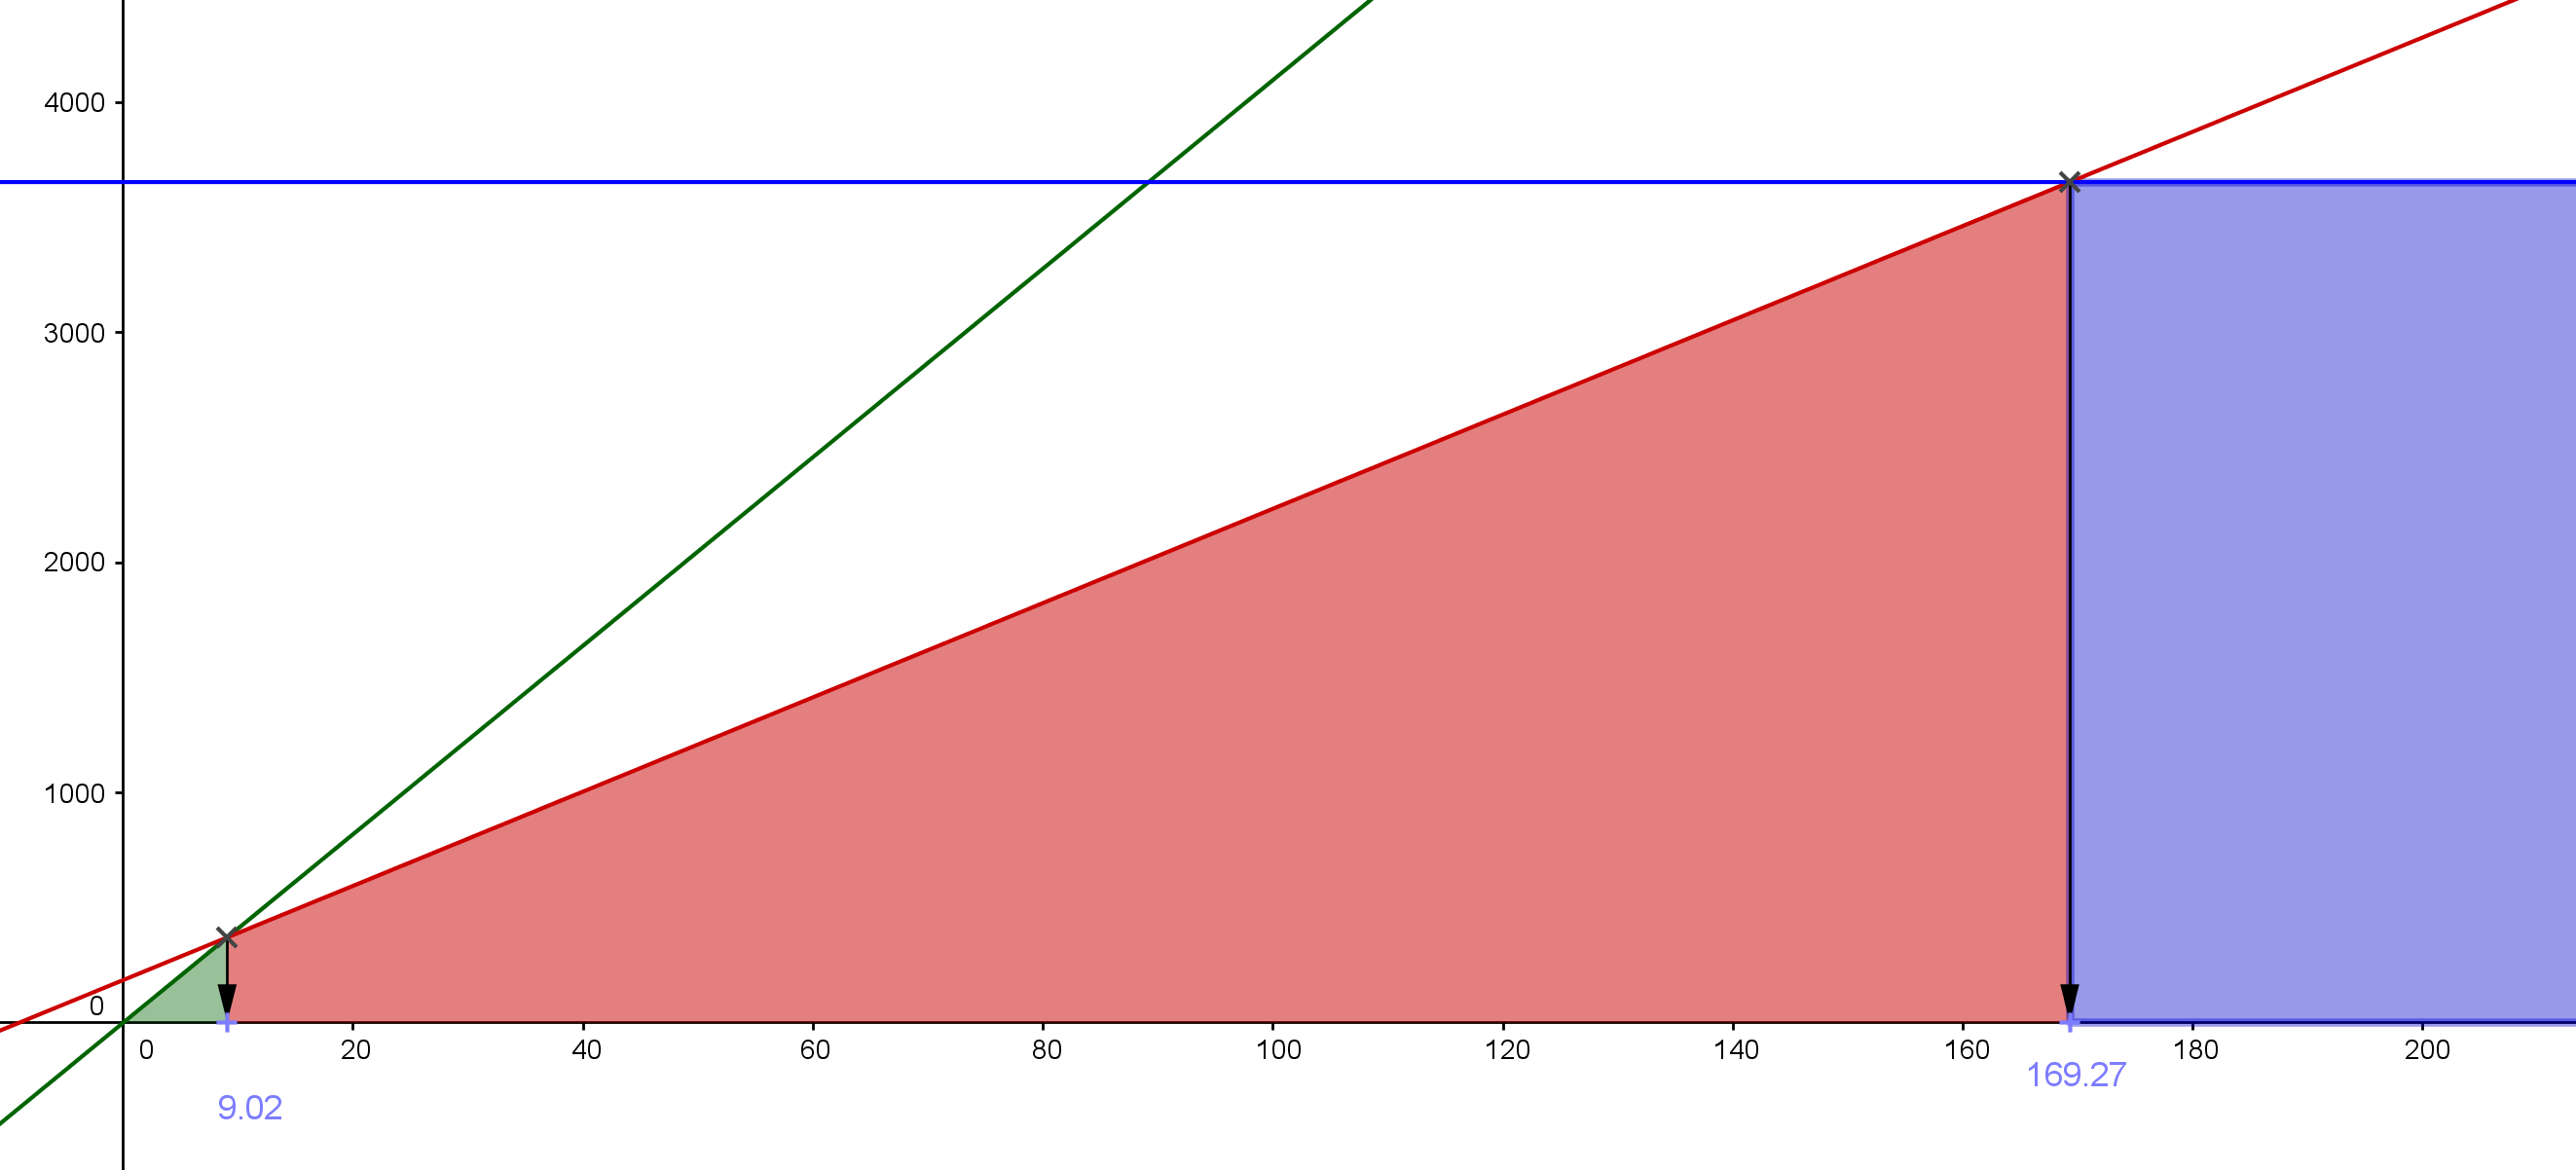
\includegraphics[width = 0.9 \textwidth]{rentabilite/comparatif.png}
\end{center}
Ainsi dans la première zone, la fonction $h$ est la plus avantageuse, la deuxième, la fonction $i$ et la dernière la fonction $j$.

Il nous faut à présent trouver les pivots des zones. On les trouve aux intersections des fonction $h$ et $i$ ainsi qu'à celle des fonctions $i$ et $j$. L'intersection des fonction $h$ et $j$ ne nous intéresse pas, comme on le voit sur le graphique.

Commençons par les fonctions $h$ et $i$ :
$$
\begin{array}{lcl}
41 x &=& \frac{41}{2} x + 185 \ssi \\
41x - \frac{41}{2}x = 185 \ssi \\
\frac{41}{2} x = 185 \ssi \\
x = \frac{370}{41} \simeq 9,02
\end{array}
$$
puis par celle des fonctions $i$ et $j$
$$
\begin{array}{lcl}
\frac{41}{2}x + 185 &=& 3655 \ssi \\
\frac{41}{2} x &=& 3470 \ssi \\
x = \frac{6940}{41} \simeq 169,27
\end{array}
$$
Ainsi si Jean-Paul effectue entre $0$ et $9$ trajets par an, il préférera payer ses trajets en plein, entre $10$ et $169$ trajets, il prendra un demi-tarif, au-delà de $170$ trajets, il prendra un abonnement général.
\end{exemple}